\section{Fonction noyau}\label{sec:kernel}

On rappelle la propriété suivante du produit scalaire pour les vecteurs $\textbf{x}$ et $\textbf{y}$ : 

$$\textbf{x}\textbf{y}^T = \textbf{x} \cdot \textbf{y}.$$

En général, lorsque le produit scalaire entre les transformations définis en (\ref{eq:featurespace}) existe, on appelle cette fonction le noyau et on peut reformuler le produit scalaire comme
$$\textrm{k}(\textbf{x}, \textbf{y}) = \Phi(\textbf{x})\Phi(\textbf{y})^T = \Phi(\textbf{x})\cdot \Phi(\textbf{y}).$$

Dans plusieurs problèmes d'apprentissage, le "truc du noyau" permet d'éviter de calculer directement les nouvelles données $\Phi(\textbf{x})$. 
En effet, il n'est parfois pas nécessaire d'avoir toutes les données car on peut reformuler les équations de mise à jour par le produit scalaire 
entre différents $\Phi(\textbf{x})$ et ainsi les remplacer par la fonction de noyau. \\

Réutilisons l'exemple fourni à la section précédente. Nous avions le jeu de donnée avec des données réparties selon 3 cercles concentriques 
et la transformation $$\Phi(\textbf{x})= (x_1^2 + \sqrt{2} \times x_1\times x_2 + x_2^2)$$. \\ la fonction noyau associée est

$$\k(\textbf{x,y})= (x \cdot y)^2$$

Concrètement, cette projection fera en sorte de créer un blocs de points de données pour chacune des classes à des hauteurs différentes. 

\begin{figure}[H]
	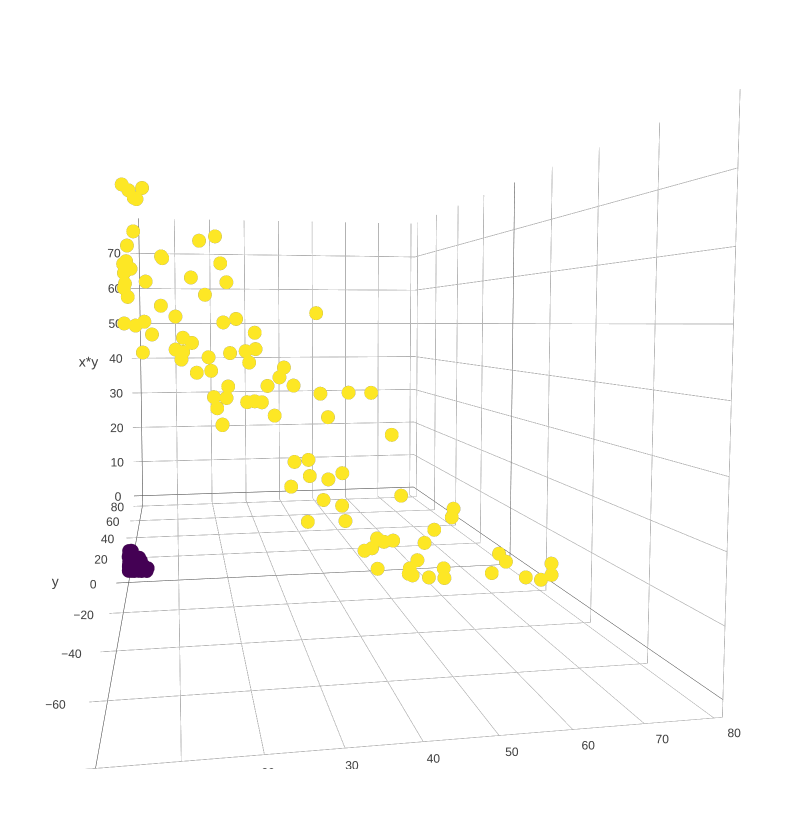
\includegraphics[width=3in]{exemple_1_3d}
\end{figure}


Cette information, 
initalement cachée du jeu de données, devient évidente lorsqu'on regarde la valeur de chaque point sur la dimension ajoutée (soit la hauteurs entre chaque groupe de points.)
Si nous utilisions le noyau associé pour gérérer des valeurs au lieu de projetter les données avec la fonction $\Phi(\textbf{x})$,
nous aurions une division des données qui serait sensiblement similaire \\ 

\begin{figure}[H]
	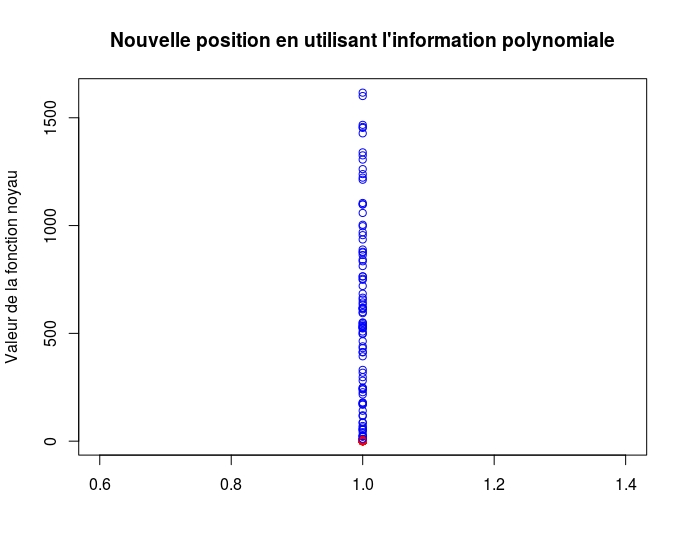
\includegraphics[width=3in]{exemple_1_kernel}
\end{figure}


Il est important de retenir que pour obtenir l’information $\textrm{k}$ générée par la projection, les transformations vers $\mathcal{F}$ n'ont pas à être explicitement calculées. 
La fonction de noyau permet de calculer directement cette information et il s’agit de la raison pour laquelle les noyaux sont des outils intéressants. \\

L'exemple jouet ne présente qu’une projection en 3 dimensions et son utilité peut sembler limité. Cependant, certains noyaux émulent une projection dans un espace de dimensions infinie. 
En projetant dans un espace ayant un nombre de dimensions infini, il est théoriquement possible de modéliser 
parfaitement chacun des points des données. On a ainsi l’assurance de trouver une fonction linéaire séparant les 
données parfaitement - sans avoir à faire des calculs qui seraient impossibles à faire.\\

En pratique, au lieu de sélectionner un espace d'attributs $\mathcal{F}$, on sélectionne directement le noyau. 
Il n'est pas nécessaire de connaître l'espace d'attributs $\mathcal{F}$ ou la fonction $\Phi$. De plus, 
il est possible que la fonction $\Phi$ projète des données vers une dimension infinie. Ceci ne cause pas de problème car 
l'impossibilité analytique de déterminer la fonction $\Phi(\textbf{x})$ est esquivée par 
le truc du noyau. Des exemples de noyaux communément utilisés sont présentés dans la table \ref{tab:kernels}.

\begin{table}[H]
	\centering
\begin{tabular}{|c|c|}
	\hline
	         Nom           &                  $k(\textbf{x}, \textbf{y})$                  \\ \hline
	    Gaussien (RBF)     & $\exp \left(\frac{-|| \textbf{x} - \textbf{y}||^2}{c}\right)$ \\ \hline
	      Polynomial       &         $((\textbf{x} \cdot \textbf{y} + \theta))^d$          \\ \hline
	     Sigmodoidal       &    $\tanh (\kappa (\textbf{x} \cdot \textbf{y}) + \theta)$    \\ \hline
	Multiquadrique inversé &     $\frac{1}{\sqrt{||\textbf{x}-\textbf{y}||^2 + c^2}}$      \\ \hline
\end{tabular} 
\caption{Noyaux communs}
\label{tab:kernels}
\end{table}
